% Student template

\clearpage

% TODO: Add offset calculation variables (pretty easy)
\providecommand\studentimages[1]{%
	\AddToShipoutPictureBG*{
		\AtTextUpperLeft{
			\put(-15, -215){\includegraphics[keepaspectratio=true, width=180pt]{parts/students/figures/#1.jpg}}
			\put(-50, -250){
\includegraphics[keepaspectratio=true, width=250pt]{ring.png}}
		}
	}

	\AddToShipoutPictureBG*{
		\AtTextLowerLeft{
			\put(\textwidth - 120, 50){\includegraphics[keepaspectratio=true, width=160pt]{parts/students/figures/#1_child.jpg}}
			\put(\textwidth - 130, 40){
\includegraphics[keepaspectratio=true, width=180pt]{rahmen.png}}
		}
	}
}

\providecommand\studentprofile[8]{%
	\sectionmark{Steckbrief - #1}

	% Steckbrief Tabelle
	\begin{tikzpicture}[overlay]
		\node[text width=250pt, align=left] at (12, -5) {
			\Large{\begin{tabular}{@{}ll@{}}
				\textbf{Name:} & #1 \\
				\textbf{Geburtstag:} & #2 \\
				\textbf{Lieblingsfach:} & #3 \\
				\textbf{Hobbies:} & #4 \\
				\textbf{Lieblingsgenre:} & #5 \\
			\end{tabular}}\\~\\
			\textbf{Das werde ich am meisten vermissen:}\\#6\\~\\
			\textbf{Ohne das hätte ich die Oberstufe nicht geschafft:}\\#7\\~\\
			\textbf{Lebensmotto:}\\#8\\~\\
		};
	\end{tikzpicture}
}

\providecommand\studenttable[2]{%
	\vskip 10cm
	\hspace*{-1.2cm}
	\Large{\begin{tabular}{@{}ll@{}}
		\textbf{Erkennungsmerkmale:} & #1 \\
		\textbf{Zukunftspläne:} & #2 \\
	\end{tabular}}
}

\providecommand\studentcomments[1]{%
	\begin{figure}[H]
		\hspace*{-2.5cm}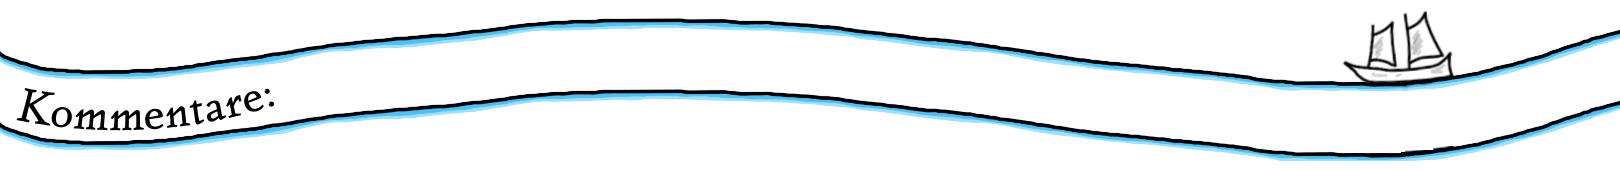
\includegraphics[keepaspectratio=true, width=\paperwidth]{mittelwelle.png}
	\end{figure}
}
